\begin{chapter}{Teoria da Pinça Ótica}
\label{cap2}

%\hspace{5 mm} BLABLABLA

\section{Introdução}

\hspace{5 mm}A presente dissertação é um resultado do trabalho do grupo de pinças óticas da UFRJ, que tem sido desenvolvido há quase duas décadas {\bf rever com Paulo->reclamou dessa frase}. Os trabalhos de teoria do grupo têm como objetivo descrever o aparato de pinças óticas, descoberta por Arthur Ashkin em 1986\cite{Ashkin1986} \cite{Ashkin1977}. Suas contribuições para o ramo de armadilhamento ótico vêm desde 1970, com seu primeiro artigo publicado sobre o assunto\cite{Ashkin1970}.
Em 2018, seus trabalhos sobre a pinça ótica e toda a sua importancia para aplicação em biologia lhe renderam o prêmio Nobel de 2018. 

A importância desse aparato exigiu uma descrição teórica satisfatória. Os primeiros modelos que tentam descrever as forças da pinça ótica fazem uso de diversas aproximações para descrever o feixe que sai da objetiva e a interação da esfera com o campo. Falarei brevemente destes na próxima seção.

O primeiro artigo publicado pelo grupo que diz respeito a teoria de pinças óticas foi em 2000 \cite{Neto2000}, e deriva a força axial (na direção $z$) na microesfera em cima do eixo para um feixe de polarização circular. Resultados seguintes estendem o anterior para uma posição arbitrária da microesfera em relação ao foco do feixe e derivam forças nas demais direções (em coordenadas cilíndricas: azimutal e radial) \cite{Mazolli2003}. O caso da polarização linear é discutido em \cite{Dutra2007}. Posteriormente, eles também inserem correções à aberração esférica em \cite{Viana2007} (para interface vidro-água no porta-amostra) e ao astigmatismo e coma em \cite{Dutra2014}.

Na seção {\bf inserir seção}, discutirei brevemente o modelo desenvolvido pelo grupo (MDSA+, do inglês Mie-Debye Spherical Aberration, com correção de outras aberrações). Este foi usado para obter os resultados da presente dissertação. Ele leva em conta diversos efeitos [CITAR EXEMPLOS] que são ignorados pelos demais, além de ser válido para um espectro maior de razões entre o comprimento de onda $\lambda$ e o raio $a$ (também chamado de parâmetro de tamanho, ou $\beta$).

%A importância de um modelo teórico derivado de primeiros principios é enorme para se entender com clareza a física de um experimento ou fenômeno. Portanto, comparar teoria e experimento é de extrema necessidade para validar tal teoria. 
%
Ajustes de dados experimentais com o modelo MDSA foram feitos e publicados pelo grupo \cite{viana_2006, kaina}. Uma vez demonstrada que a teoria tem boa concordância com o experimento, podemos tentar prever parâmetros experimentais a partir dela. Esse é um dos objetivos do presente trabalho, e, para tal, discutiremos nas próximas seções um pouco sobre o modelo Mie-Debye e suas extensões. Esse tema ja foi abordado em teses de doutorado de ex-alunos do grupo \cite{Mazolli, Rafael}, que tomaremos e recomendamos como referência para este texto.

O modelo MD levam em conta um efeito que a princípio não se apresenta com clareza: a interação de momento angular de spin e orbital do feixe. A alta abertura numérica da objetiva e o espalhamento Mie são dois elementos importantes levados em consideração e que são responsáveis por efeitos de conversão de momentos angulares\cite{Bliokh2015}. Faremos uma breve discussão nesse capítulo sobre esses efeitos, a fim de elucidar não só os mesmos, mas os resultados obtidos nas simulações e no experimento. ({\bf rever esse paragrafo})

%
%
%%%%%  Seção 1  %%%%%
%
%
\section{Modelo Mie-Debye}

\hspace{5 mm}Discutiremos brevemente nesse capítulo o modelo MDSA+. Para entender a orígem das expressões para a força, vamos começar do problema mais simples. Trataremos nessa seção as bases do modelo Mie-Debye, para uma onda de polarização circular (direita ou esquerda). Os detalhes de tais cálculos podem ser encontrados em \cite{mazolli}, e não estarão no presente trabalho para evitar repetição. 

Começamos pela forma como se faz o cálculo da força em uma amostra na pinça ótica \cite{jackson}:

\begin{equation}
\vec{F} = \oint_{\sigma} \hat{n} \cdot T d \sigma - \mu \epsilon \frac{d}{dt} \int_{\nu} \vec{S} d \nu,
\label{2_F}
\end{equation}

onde $\sigma$ é uma superfície que envolve a amostra na pinça ótica, $\nu$ é o interior dessa superfície, $T$ é o tensor das tensões de Maxwell e $\mu$ e $\epsilon$ são a permeabilidade magnética e a permissividade elétrica do meio envolvendo a amostra, respectivamente. 

O primeiro passo, portanto, é calcular o campo eletromagnético incidente e espalhado nessa amostra (centro espalhador). O campo incidente na amostra tem formato cônico sólido, gerado pela objetiva. Montaremos esse campo superpondo ondas planas. Para tanto, começamos tratando do caso de uma onda plana se propagando na direção $z$, com polarização circular. Essa é a polarização conveniente para expansão do campo em multipolo (ondas esféricas ou ondas parciais). Outros casos de polarização serão discutidos adiante. A base de multipolos é a ideal para problemas com simetria esférica, pois são compostas pelos harmônicos esféricos na parte radial, que são autofunções dos operadores de momento angular $L^2$ e $L_z$. Esse fato será importante para obter os campos vetoriais a partir dos potenciais de Debye, que serão definidos a seguir: 

\begin{equation}
\Pi^{E}=\sum\limits_{J} \Pi^{E}_J=\sum\limits_{J}\frac{ ({\mathbf r}\cdot{\mathbf E })_J }{J(J+1)} \qquad e\qquad \Pi^{M}=\sum\limits_{J} \Pi^{M}_J=\sum\limits_{J}\frac{ ({\mathbf r}\cdot{\mathbf H })_J }{J(J+1)} .
\label{debye_def}
\end{equation}
%
com

\begin{equation}
{\mathbf E}=E_0(\hat{x}\pm i \hat{y})e^{ikz-i\omega t} \qquad e\qquad {\mathbf H}=\frac{n_1}{\mu c}(\mp i){\mathbf E}.
\label{onda_plana}
\end{equation}
%
onde $n_1$ é o índice de refração do meio ao redor da amostra. Tais potenciais serão úteis para resolver o problem do espalhamento Mie. Estes decompõem os campos em dois modos, um deles com o campo ${\mathbf E}$ paralelo à superfície do objeto espalhador ($\Pi^{M}$, modo transversal elétrico) e outra perpendicular ($\Pi^{E}$, modo transversal magnético). Essa decomposição forma a base para se aplicar as condições de contorno e obter os coeficientes de Mie, que podemos entender como as amplitudes de espalhamento de cada onda parcial. Os coeficientes de Mie para o espalhamento são:

\begin{equation}
a_J=\frac{\psi_J(\beta)\psi'_J(\alpha)-N\psi'_J(\beta)\psi_J(\alpha)}{\zeta^{(1)}_J(\beta)\psi'_J(\alpha)-N\zeta'^{(1)}_J(\beta)\psi_J(\alpha)} \qquad e\qquad
b_J=\frac{\psi'_J(\beta)\psi_J(\alpha)-N\psi_J(\beta)\psi'_J(\alpha)}{\zeta'^{(1)}_J(\beta)\psi_J(\alpha)-N\zeta^{(1)}_J(\beta)\psi'_J(\alpha)},
\label{mie}
\end{equation} 
%
onde $\beta=ka$, $\alpha=Nka$, $a$ é o raio da esfera, $\psi_J=xj_J(x)$ e $\zeta^{(1)}_J=xh^{(1)}_J(x)$ são as funções de Bessel-Riccati e $j_J(x)$ e $h^{(1)}_J(x)$ são as funções esféricas de Bessel e Henkel, respectivamente. Os campos espalhados provenientes de $\Pi^E$ e $\Pi^M$ terão os termos $a_J$ e $b_J$ respectivamente multiplicando as expressões dentro dos somatórios em $J$.

Assim, uma vez encontradas as soluções escalares para os campos espalhados e incidentes, temos que reobter os campos vetoriais. Fazemos isso usando um conjunto de operadores vetoriais que comutam com $\nabla ^2$ e são perpendiculares entre si: $-i {\mathbf r}\times\nabla = {\mathbf L}$,$\nabla \times {\mathbf L}$ e $\nabla$. No espaço de Fourier, esses operadores são proporcionais a ${\mathbf k}\times \nabla_{\mathbf k}$, ${\mathbf k}\times({\mathbf k}\times \nabla_{\mathbf k}) \propto \nabla_{\mathbf k}$ e ${\mathbf k}$, respectivamente. A figura \ref{vet_fourier} mostra os vetores em questão. O operador ${\mathbf k}$ fornece a soluções com campos na direção de propagação, ou seja, campos com divergência não nula e que não são soluções do nosso problema.
%
\begin{figure}[h]
\begin{center}
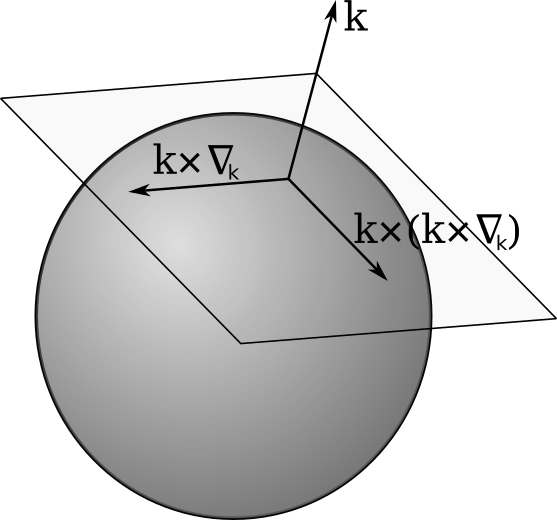
\includegraphics[scale=0.5]{vec_fourier}
\caption{Operadores vetoriais no espaço de Fourier usados para encontrar as soluções vetoriais.}
\label{vet_fourier}
\end{center}
\end{figure}
%
Obtemos, até então, os potenciais de ondas planas incidentes e espalhadas na direção $z$ em coordenadas esféricas. Queremos usa-las para montar um feixe cônico de alta abertura numérica. Faremos isso rotacionando e superpondo diversas ondas planas usando o operador ${\mathbf J}$, que é o gerador de rotações no espaço. Como a dependência angular dos potenciais de Debye estão contidas nos harmôncos esféricos, o procedimento se resume em fazer a rotação dos mesmos. Usando o operador $D(\alpha,\beta,\gamma)=e^{-i\alpha J_z}e^{-i\beta J_y}e^{-i\gamma J_z}$ e o fato de que os harmônicos esféricos são autofunções de $J_z$, obtemos:

\begin{equation}
Y_{JM}(\theta',\phi')=\sum \limits_{M'=-J}^{J} Y_{JM'}(\theta,\phi) e^{-i(\alpha M'+\gamma M)} d^J_{M'M}(\beta),
\label{harm_esf_rot}
\end{equation}
%
que representa um harmônico esférico em um eixo rodado com coordenadas $\theta'$ e $\phi'$, onde $d^{J}_{M',M}(\beta)=e^{-i\beta J_y}$ é o elemento da matriz-$d$ de Wigner e  $\alpha$, $\beta$, e $\gamma$ são os ângulos de Euler. A rotação é feita de forma que o eixo $z$ coincida com o eixo $\hat{{\mathbf k}}$ de propagação. Para isso, $\alpha =\phi_k$ e $\beta =\theta_k$. Usamos o último ângulo de Euler para determinar corretamente a direção de polarização do feixe fazendo $\gamma =-\phi_k$. Substituindo em \ref{debye_def}, os potenciais de Debye rotacionados ficam:

\begin{equation}
\Pi^E =\pm \frac{E_0 e^{-i\omega t}}{k}\sum \limits_{J=1}^{\infty}(i)^{J+1}j_J(kr)\sqrt{\frac{4\pi(2J+1)}{J(J+1)}} \sum \limits_{M'=-J}^J e^{i\phi_k(M'\mp1)}d^J_{M',\pm1}(\theta_k)Y_{JM'}(\theta,\phi),
\label{debyeE_rot}
\end{equation}
e
\begin{equation}
\Pi^M =\frac{H_0 e^{-i\omega t}}{k}\sum \limits_{J=1}^{\infty}(i)^{J}j_J(kr)\sqrt{\frac{4\pi(2J+1)}{J(J+1)}} \sum \limits_{M'=-J}^J e^{i\phi_k(M'\mp1)}d^J_{M',\pm1}(\theta_k)Y_{JM'}(\theta,\phi).
\label{debyeM_rot}
\end{equation}
%

O próximo passo é integrar no ângulo solido do cone. Começando pela varável $\phi_k$ (ou seja, componente $\phi$ da direção do vetor de onda ${\mathbf k}$; notação que será usada para $\theta_k$ também), obtemos:

\begin{equation}
\begin{split}
\Pi^E_{\theta_k} =\pm \frac{E_0 e^{-i\omega t}}{k}\sqrt{\cos(\theta_k)}\sum \limits_{J=1}^{\infty}(i)^{J+1}j_J(kr)\sqrt{\frac{4\pi(2J+1)}{J(J+1)}} \times \\ \times \sum\limits_{M'=-J}^J d^J_{M',\pm1}(\theta_k)Y_{JM'}(\theta,\phi) \int\limits_0^{2\pi} d\phi_k e^{-i\phi_k(M'\mp1)} ,
\label{pi_phi}
\end{split}
\end{equation}
%
onde o termo $\sqrt{\cos(\theta_k)}$ vem da condição do seno de Abbe. O cone sólido se obtem integrando em $\theta_k$:

\begin{equation}
\begin{split}
\Pi^E=\int\limits_0^{\theta_0}d\theta_k \sin\theta_k \Pi^E_{\theta_k}, \\
\Pi^M=\int\limits_0^{\theta_0}d\theta_k \sin\theta_k \Pi^M_{\theta_k},
\label{integral_theta}
\end{split}
\end{equation}
%
onde $\theta_0$ é a meia abertura do feixe.

Para derivar a força na microesfera em função da sua posição relativa ao foco do feixe, temos que calcular os campos deslocados em relação ao centro do objeto espalhador, ou seja, a orígem. Fazemos isso usando o gerador de translações no espaço ${\mathbf k}$, com o operador $e^{-i{\mathbf k}\cdot{\mathbf R}}$, onde ${\mathbf R}=q_x\hat{x}+q_y\hat{y}+q_z\hat{z}$ é o vetor de deslocamento. Multiplicamos esse operador em cada coeficiente de multipolo, e dessa forma, o operador fica dentro da integral em $\phi_k$, que leva ao seguinte resultado:

\begin{equation}
\begin{split}
\int\limits_0^{2\pi} d\phi_k e^{-i{\mathbf k}\cdot{\mathbf R}} e^{-i\phi_k(M'\mp1)}=e^{-ik z\thinspace \cos\theta_k} 2\pi(-i)^{M'\mp1}J_{M'\mp1}\left(k\sin\theta_k\sqrt{q_x^2+q_y^2}\right)e^{-i(M'\mp1)\phi}.
\end{split}
\end{equation}
%

Uma vez determinados os potenciais de Debye incidentes e espalhados, podemos obter os campos aplicando os operadores $-i\nabla\times{\mathbf L}$ e $-i{\mathbf L}$:

\begin{equation}
\begin{split}
{\mathbf E}_T={\mathbf E}_{IN}+{\mathbf E}_{S}=-i\nabla\times{\mathbf L}(\Pi^E_{IN}+\Pi^E_S)+i \omega \mu(-i){\mathbf L}(\Pi^M_{IN}+\Pi^M_S), \\
{\mathbf H}_T={\mathbf H}_{IN}+{\mathbf H}_{S}=-i\nabla\times{\mathbf L}(\Pi^M_{IN}+\Pi^M_S)-i \omega \epsilon(-i){\mathbf L}(\Pi^E_{IN}+\Pi^E_S).
\end{split}
\end{equation}
%

Finalmente, calculando a integral \ref{2_F}, obtemos a força na microesfera de um campo cônico e com perfil de instensidade constante antes de entrar na objetiva. Essa integral pode ser resolvida tomando a superfície $\sigma$ como uma esfera (com centro na orígem) com raio tendendo a infinito. Isso faz com que as componentes radiais do campo sejam desprezadas no cálculo, pois caem com $\frac{1}{r^2}$, comparado às componentes tangenciais que caem com $\frac{1}{r}$. Temos, então:

\begin{equation}
{\mathbf F}=\frac{-1}{2}r\left( \int d\Omega (\epsilon E^2_{tan}{\mathbf r}) + \int d\Omega (\mu H^2_{tan}{\mathbf r}) \right),
\end{equation}
%
onde as duas integrais dentro do parentesis são iguais. Sendo assim, a força vai depender do quadrado dos campos ($E^2$ e $H^2$), e de termos proporcionais a ${\mathbf E}_{IN}\cdot{\mathbf E}_{IN}^*$(incidente-incidente), $Real({\mathbf E}_{IN}\cdot{\mathbf E}_S^*)$(espalhado-incidente) e ${\mathbf E}_S\cdot{\mathbf E}_S^*$(espalhado-espalhado). O primeiro desses termos (campo incidente-incidente) não contribui para a força, pois trata-se do caso onde não há centro espalhador. O produtos dos campos espalhado-incidente é chamado termo de extinção, e representa a taxa de perda de momento do campo incidente para o centro espalhador. Por fim, o termo de espalhamento (espalhado-espalhado) é menos a taxa de transferência de momento para o campo espalhado.

A expressão para a força será mostrada depois de introduzirmos o perfil do feixe e a polarização, uma vez que tanto os campos mudam, quanto as expressões da força ganham termos adicionais. Junto com a expressão para a força, serão mostrados os coeficientes de multipolo $\G_JM$, que carregam as informações de aberrações e do perfil de intensidade.

\section{Efeito do perfil gaussiano}

\hspace{5 mm}O efeitos do perfil gaussiano no feixe. Faremos isso analisando o campo paraxial na entrada da obejtiva. Trataremos também do efeito da aberração esférica causada pela objetiva quando a lente é imersa em um meio com índice de refração diferente do meio que envolve a microesfera. 

Para introduzir o efeito que o perfil do feixe produz, basta saber como é o feixe paraxial antes de ser focalizado. Primeiramente, assumimos que tal feixe incidente esteja com a altura da cintura mínima coincidente com a entrada da objetiva. Isso nos permite tratar-lo como um feixe cilíndrico (de raio de curvartura infinito). {\bf colocar discussão sobre feixe paraxial em algum apendice, e fazer a referencia aqui.} O campo fica:

\begin{equation}
{\mathbf E}_{IN}^{antes}(\vec{r},t)=E_0 e^{ikz} e^{-\frac{f^2\sin^2\theta_k}{\omega_0^2}}(\hat{{\mathbf x}}\pm i\hat{{\mathbf y}}) e^{i\omega t},
\label{campo_ent}
\end{equation}
%
onde $\omega_0$ é a cintura (waist) mínima, $f^2\sin^2\theta_k=\rho^2$ (pela condição do seno) é a distância ao eixo do feixe ao quadrado. Ao passar pela objetiva, o campo também ganha uma correção de efeitos de difração \cite{RICHARDSeWOLF}, o fator multiplicativo $-i\frac{f}{\lambda}$. O fator $e^{-\frac{f^2\sin^2\theta_k}{\omega_0^2}}$ deve ser inserido dentro da integral em $\theta_k$. Assim, as expressões para os multipolos \ref{integral_theta} são alteradas.

\section{Efeitos de polarização}

\hspace{5 mm}Entender o caso de polarização linear vai tornar possível a compreensão do caso de polarização elíptica. Começamos modelando o feixe como uma superposição de polarização circular a direita a e esquerda, com pesos iguais. O único procedimento que muda em relação ao caso de polarização circular é quando tomamos os quadrados dos campos ${\mathbf E}$ e ${\mathbf H}$. Teremos campos espalhados e incidentes de ambas as polarizações, com as quais montamos os respectivos potenciais de Debye. Produtos de campos de mesma polarização serão chamados puros, e produtos de campos de polarização oposta serão chamados cruzados. Introduzimos, então, o fator de eficiencia vetorial, também chamado de força normalizada, para o feixe de polarização linear:

\begin{equation}
{\mathbf Q} = \frac{\left<{\mathbf F}\right>}{n_1 P/c}= \frac{1}{2}{\mathbf Q}^{(\sigma +)} + \frac{1}{2}{\mathbf Q}^{(\sigma -)} + {\mathbf Q}^{({\it cross})}
\end{equation}
%
onde $\left<{\mathbf F}\right>$ é a média temporal da força, $c$ é a velocidade da luz no vácuo e P é a potencia do feixe incidente na amostra. Os termos ${\mathbf Q}^{(\sigma \pm)}$ são os termos que encontraríamos para a polarização circular direita ou esquerda. O termo ${\mathbf Q}^{({\it cross})}$ é o que chamamos de cruzado. 

A força exercida por uma polarização elípitica pode ser obtida introduzindo a dependência com o ângulo da placa de quarto de onda (PQO, ou QWP) no feixe paraxial incidente na entrada da objetva:

\begin{equation}
{\mathbf E}^{ent}(\rho,\phi,z) = E_{centro} e^{ik_0z} e^{\frac{-\rho^2}{w_0^2}} \sum \limits_{\sigma = +1,-1} \frac{1 - ie^{-2i\sigma \theta}}{2} \hat{\bf{\epsilon}}_\sigma .
\label{l}
\end{equation}
%
Dessa forma, os potenciais de Debye ganham um termo a mais devido ao ângulo da placa de quarto de onda. Podemos, então, identificar 4 tipos de termos nas forças: diretos ou puros devidos as polarizações $\sigma_\pm$, e termos cruzados com os produtos $\sigma_\pm^*\cdot\sigma_\mp$.

\section{Aberração esférica}

\hspace{5 mm}A aberração esférica surge sempre que há algum tipo de feixe focalizado atravessando a interface de meios com índices de refração diferentes. Isso é fácil de mostrar em uma abordagem de ótica de raios e a lei de Snell. Componentes do feixe no meio com índice $n$ que incidem na interface com ângulo $\theta$, por refração, são transmitidos com um ângulo $\theta_1$ no meio com índice de refração $n_1$, de forma a respeitar a lei de Snell:

\begin{equation}
n\sin\theta=n_1\sin\theta_1.
\label{snell}
\end{equation}
%
Fica claro, então, que para um feixe focalizado incidindo perpendiculamente à interface, raios que incidem em direções com ângulo $\theta\ne 0$, ao mudarem de meio, não mais se encontram no foco. Portanto, a região de maior intensidade não se localiza mais no ponto focal, e sim difundida e mais próxima à interface ({\bf inserir figura}). Isso faz com que a posição de equilíbro da microesfera se desloque para mais perto da interface, o que pode ser entendido como um efeito de força de gradiente.

Para modelar a passagem de um meio para outro, levamos em conta a amplitude de transmissão de cada componente ${\mathbf k}$ do campo, dada por \cite{Viana2007}:

\begin{equation}
T(\theta)=\frac{2\cos\theta}{\cos\theta + N\cos\theta_1} ,
\label{transmitancia}
\end{equation}
%
onde, por \ref{snell}, $\theta_1=\arcsin(\frac{\sin\theta}{N})$, com $N=\frac{n_1}{n}$. Ao serem refratadas, as componetes de onda-plana ganham também uma fase $e^{i\Psi(z, \theta)}$, onde

\begin{equation}
\Psi(z,\theta)=k\left( -\frac{L}{N^2}\cos\theta +(L+z)\cos\theta_1 \right) 
\label{faseSA}
\end{equation}
%
é a função de aberração esférica.


\section{Interação Spin-Órbita.}

YADA

\end{chapter}